The figure below shows the results for propagation of a square wave
front in a void to the right. The standard Galerkin FEM scheme produces unphysical
oscillations and negativities, which are remedied by the FCT scheme without
introducing the amount of diffusion required by the low-order scheme. The
high-order scheme based on entropy viscosity mitigates the formation of
oscillations but ultimately still produces some negativities, but the
FCT scheme removes these.

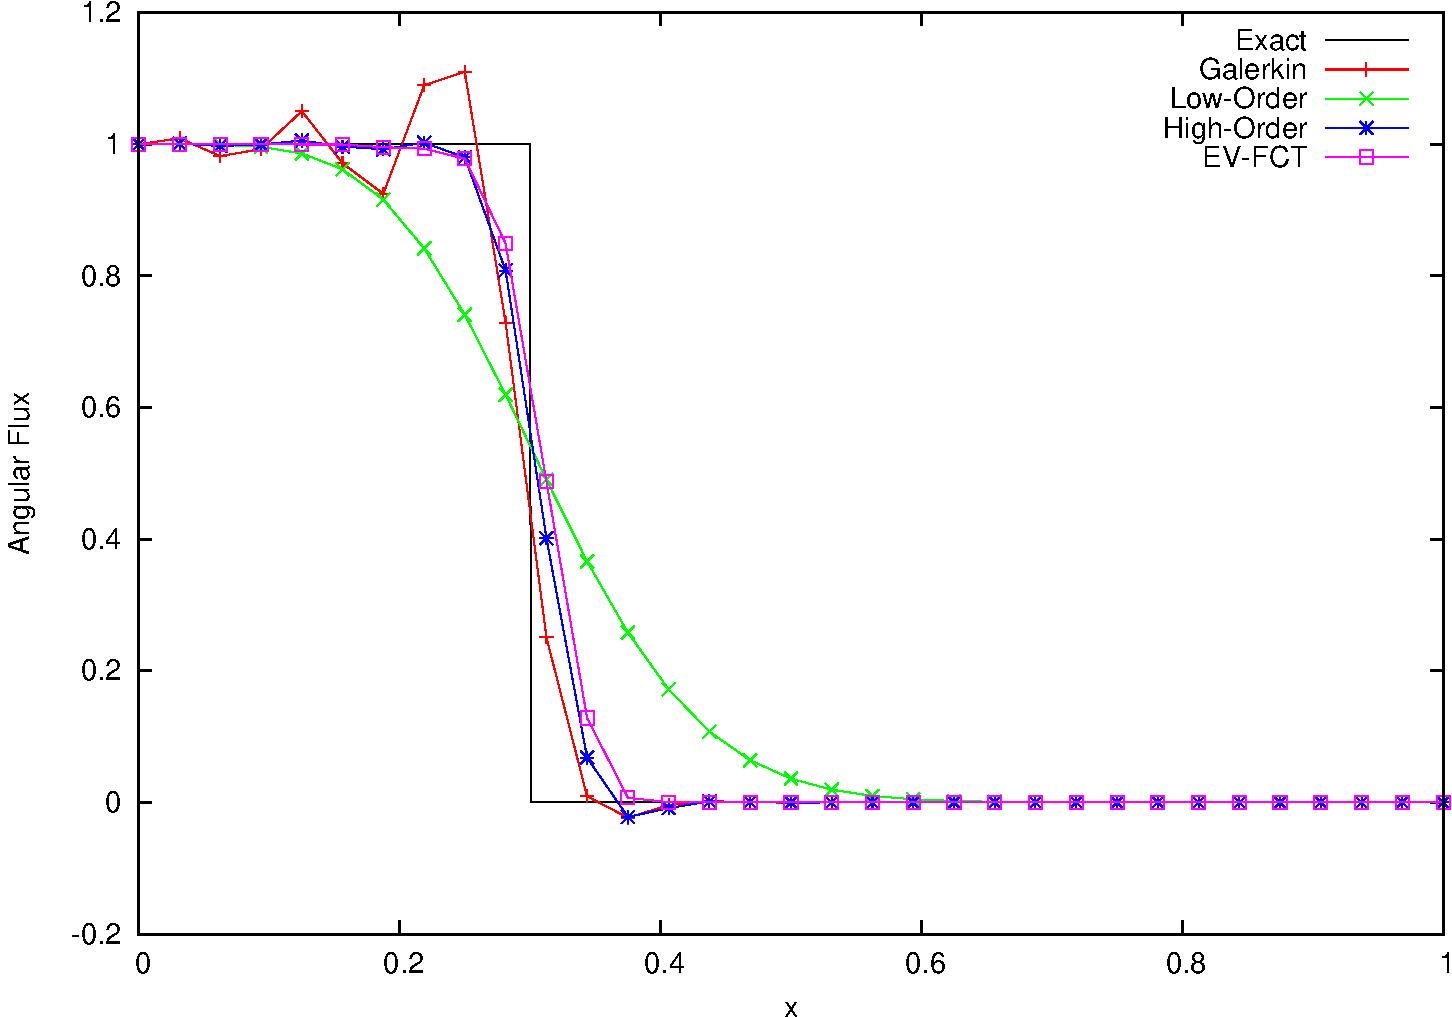
\includegraphics[width=0.20\textwidth]{figures/solutions_3_SSPRK33.pdf}

The given scheme is equally valid for multidimensional problems:
\vspace{\baselineskip}

\begin{minipage}[t]{0.5\linewidth}
  \centering
  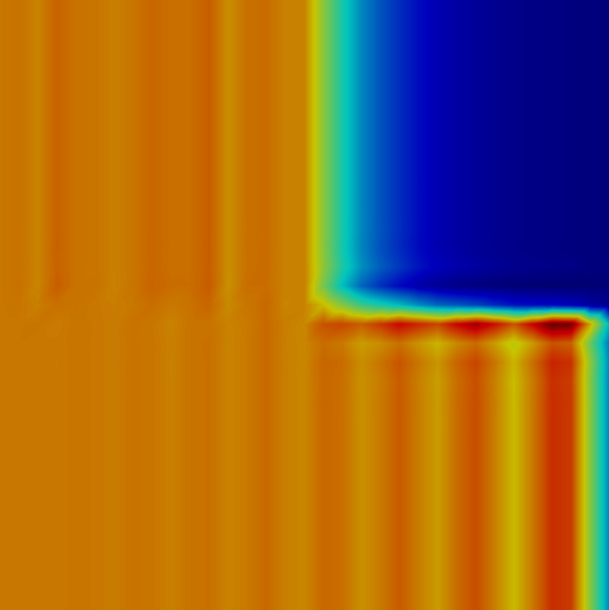
\includegraphics[width=\columnwidth]{figures/Gal2d.png}
  Galerkin
\end{minipage}
\begin{minipage}[t]{0.5\linewidth}
  \centering
  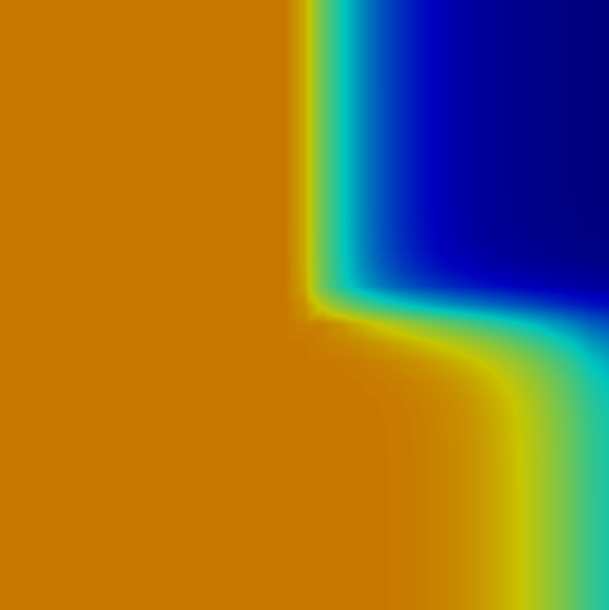
\includegraphics[width=\columnwidth]{figures/GalFCT2d.png}
  FCT
\end{minipage}

\begin{minipage}[t]{0.5\linewidth}
  \centering
  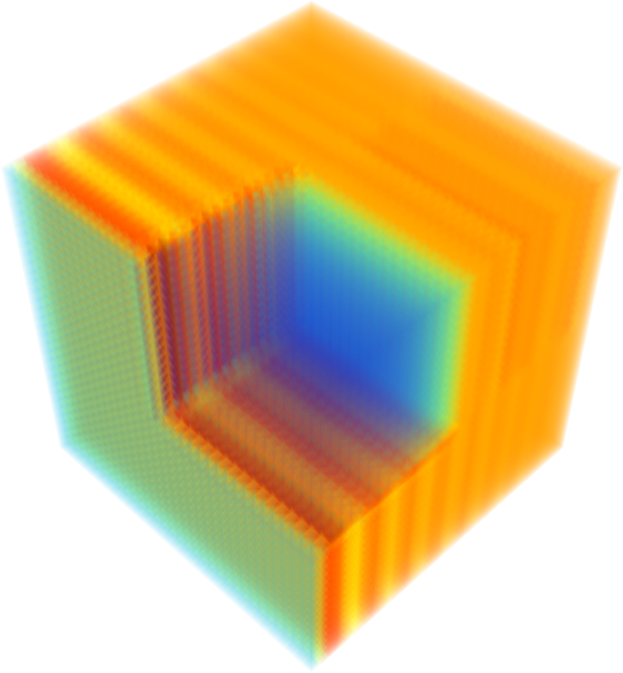
\includegraphics[width=\columnwidth]{figures/Gal_3D.png}
  Galerkin
\end{minipage}
\begin{minipage}[t]{0.5\linewidth}
  \centering
  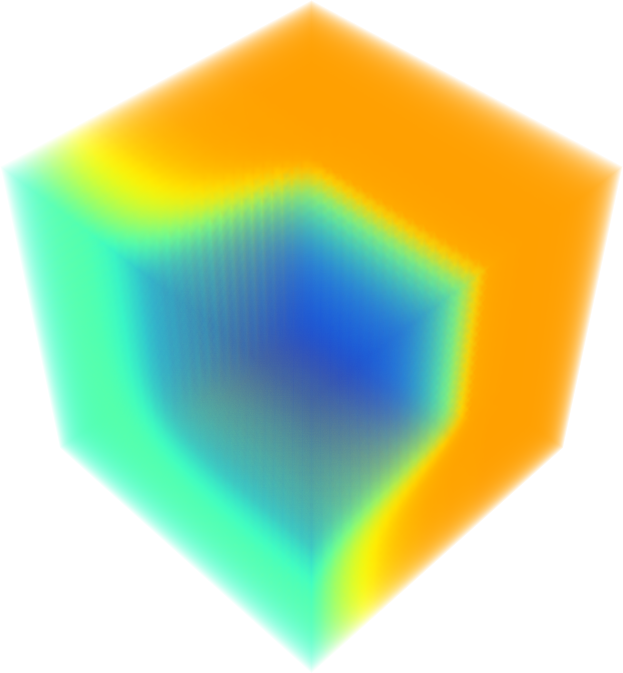
\includegraphics[width=\columnwidth]{figures/GalFCT_3D.png}
  FCT
\end{minipage}
